\section{Model Verification}\label{sec:modelVerification}
The parameters used in the final model are taken form a previous work on the boat \cite{thesis}. They are as follows:

\begin{table}[H]
    \begin{tabular}{|c|c|c|}    
        \hline %-----------------------------------------------------------------------------------
        \textbf{Parameter} &\textbf{Value} & \textbf{Units} \\
        \hline %-----------------------------------------------------------------------------------
        $m$  & 13 & kg \\
        $d_{\dot{x}_\mathrm{b}}$  & 2.86 & Nsm$^{-1}$ \\
        $d_{\dot{y}_\mathrm{b}}$  & 32.5 & Nsm$^{-1}$ \\
        $I_\mathrm{x}$  & 0.0654 & kgm$^2$ \\
        $I_\mathrm{y}$  & 1.0892 & kgm$^2$ \\
        $I_\mathrm{z}$  & 1.1067 & kgm$^2$ \\
        $d_{\dot{\phi}}$ & 0.1094 &  Nmsrad$^{-1}$\\
        $d_{\dot{\theta}}$ & 7.2030 & Nmsrad$^{-1}$ \\
        $d_{\dot{\psi}}$ & 0.2228 & Nmsrad$^{-1}$ \\
        $l_1$ & 0.05 & m \\
        $l_2$ & 0.05 & m \\
        $\rho g V \overline{GM_{T}}$ & 6.9736 & Nm\\
        $\rho g V \overline{GM_{T}}$ & 131.8316 & Nm\\
        \hline %-----------------------------------------------------------------------------------
    \end{tabular}
\end{table}

As it can be seen, the parameters corresponding to the $z_\mathrm{b}$ direction are not presented, since that equation is not used neither for the control design nor for the sensor fusion.

To verify the model a test is carried out. Two constant but different forces are applied to see the turning behavior of the real vessel, see \autoref{app:modelVerification}.

The data is then compared to the simulated model, and the results can be seen in \autoref{fig:turn} and \ref{fig:turn_time}.

\begin{figure}[H]
    \captionbox 
    {   
        Position of the boat in the $x_\mathrm{n}$-$y_\mathrm{n}$ plane given by the model simulation and the GPS data.
        \label{fig:turn}
    }                                                                 
    {                                                                  
        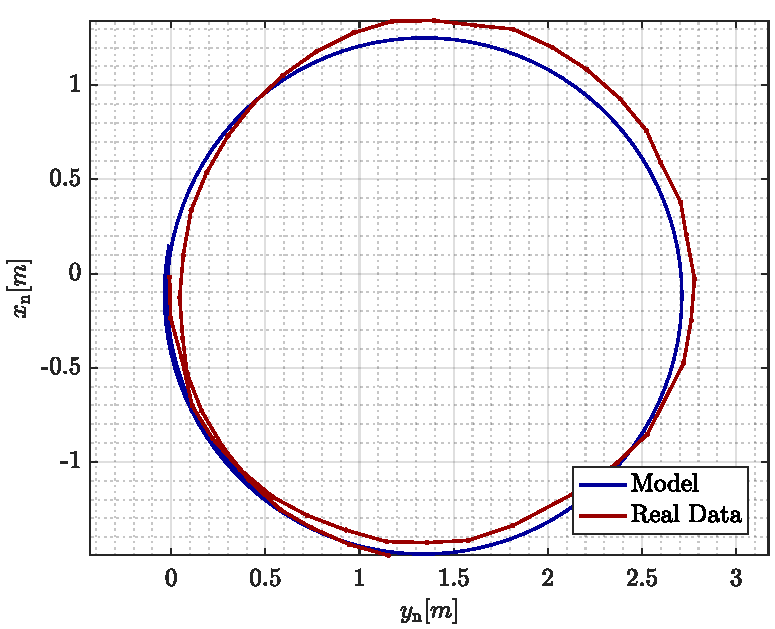
\includegraphics[width=.45\textwidth]{figures/turn}         
    }                                                                    
    \hspace{5pt}                                                          
    \captionbox  
    {      
        $x_\mathrm{n}$ and $y_\mathrm{n}$ with respect to time, both simulated and real.
        \label{fig:turn_time}
    }                                                                        
    {
        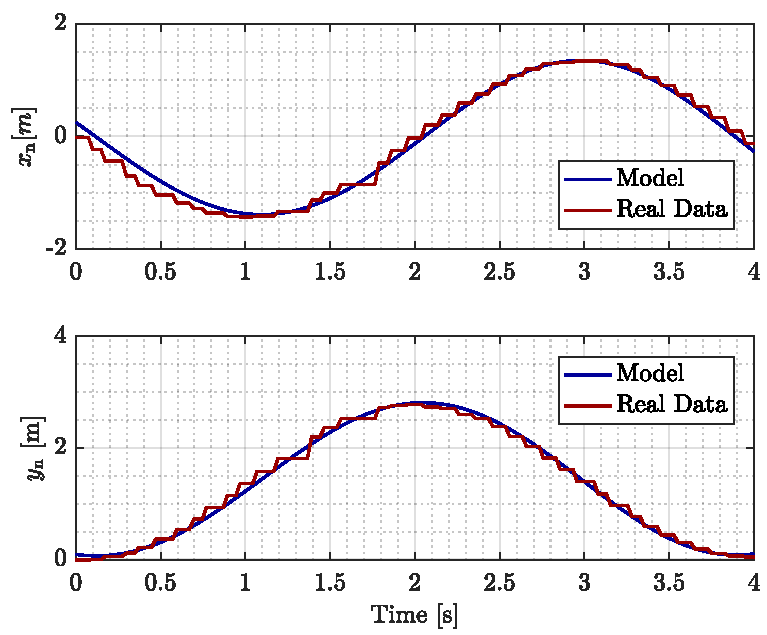
\includegraphics[width=.45\textwidth]{figures/turn_time}
    }
\end{figure}

The results show that the behavior of the real vessel is close to the simulated model. It is noticeable that the error between the model and the  real behavior mainly comes from the quantization that comes from the sampling of the gps data. Considering this comparison, the model of the vessel is deem sufficient both for simulation and control design purposes. 
